\documentclass[table]{beamer}
\usepackage{mdwlist}
\usepackage{multirow}
\usepackage{graphicx}
\usepackage{verbatim} % For using /begin{comment}; /end{comment}

\definecolor{oj}{rgb}{1.0,0.65,0.0}
\definecolor{cblue}{rgb}{0.39,0.58,0.93}

\setbeamercolor{normal text}{bg=black, fg=white}
\setbeamercolor{title}{fg=oj}
\setbeamercolor{frametitle}{fg=oj}
\setbeamercolor{block title}{fg=green}
\setbeamercolor{itemize item}{fg=cblue} % all frames will have red bullets
\setbeamercolor{enumerate item}{fg=cblue} % all frames will have red bullets

\usefonttheme{serif}
\setbeamerfont{frametitle}{series=\bfseries} % Frame titles should be bold

\title{\textbf{Coronal Seismology}}
\subtitle{\textbf{ASTR 598}}
\date{\textbf{Spring 2016}}
%\author{\textbf{Laurel Farris}}
\author{\textbf{Laurel Farris}}

\begin{document}

{\usebackgroundtemplate{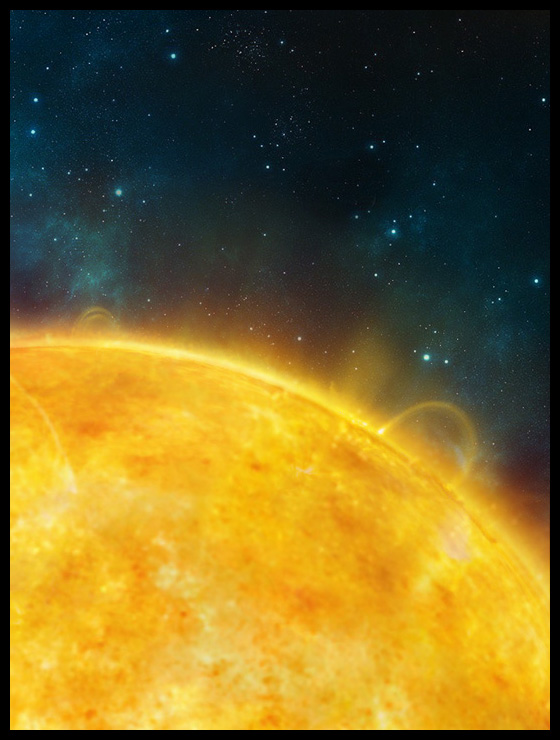
\includegraphics[width=\paperwidth]
    {awesome.jpg}}
\begin{frame}
    \titlepage
\end{frame}}

\begin{frame}{Overview}
    The body of the frame
\end{frame}

\begin{frame}{Motivation/Main Scientific Question}
    \begin{itemize}
        \item The coronal heating problem
    \end{itemize}
\end{frame}

\begin{frame}{Basic Wave stuff}
    Types of waves/oscillations:
    \begin{itemize*}
        \item Alfv\'en
        \item fast $C_{A_0} < C_{fast} < C_{A_e} $
        \item slow (acoustic) $C_{T_0} < C_{slow} < C_{s_0} $
    \end{itemize*}
    Modes:
    \begin{itemize*}
        \item Kink
        \item Sausage
        \item Acoustic
    \end{itemize*}
\end{frame}

\begin{frame}{Basic MHD equations}
    Maybe$\ldots$ See Aschwanden 6.1.3
\end{frame}

\begin{frame}
    \begin{figure}
        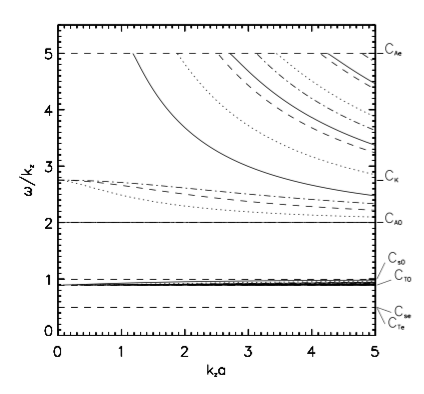
\includegraphics[width=3in]{disp_diagram.png}
    \end{figure}
\end{frame}

\begin{frame}{Instabilities}
$ \xi(x) = \xi(r)e^{i(kz+m\phi)}  $
\begin{columns}
    \begin{column}{0.33\textwidth}
    Kink
    \begin{itemize}
        \item fast magnetoacoustic waves
        \item m = 1
        \item low plasma $\beta$
        \item present in coronal loops
    \end{itemize}
    \end{column}
    \begin{column}{0.33\textwidth}  %%<--- here
    Sausage
        \begin{itemize}
            \item m = 0
        \end{itemize}
    \end{column}
    \begin{column}{0.33\textwidth}  %%<--- here
    Helical/Torsional?
    \end{column}
\end{columns}
\end{frame}

\begin{frame}{Kinks and Sausages}
    \begin{figure}
        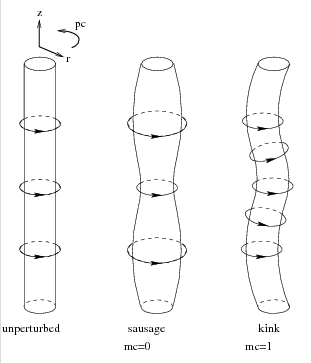
\includegraphics[width=3in]{kink_saus.png}
        \caption*{\tiny image credit:
            $https://inspirehep.net/record/1088737/files/figures_instab_locations.png$}
    \end{figure}
\end{frame}


\begin{frame}{Kink1: Coronal loop oscillations observed with the
        \emph{Transition Region And Coronal Explorer (TRACE)}}
    \begin{itemize}
        \item Gaussian vs.\ exponential
        \item Plasma motions around footpoints of coronal loops
    \end{itemize}
\end{frame}

\begin{frame}{Kink2: Excitation and damping of broadband kink waves
    in the solar corona}
\end{frame}

\begin{frame}{Sausage1: Observations of sausage modes in magnetic pores}
\end{frame}

\begin{frame}{Sausage2: Sausage waves in transversely nonuniform
    monolithic coronal tubes}
\end{frame}

\begin{frame}{Important Properties}
    \begin{center}
        \begin{tabular}{c|c|c|c|}
            \cline{2-4} & \textbf{timescale} & \textbf{sizescale} & 
                \textbf{obs.\ method}\\
            \hline \multicolumn{0}{|c|}{kink osc} & value & value & value\\
            \hline \multicolumn{0}{|c|}{sausage osc} & value & value & value\\
            \hline \multicolumn{0}{|c|}{acoustic osc} & value & value & value\\
            \hline \multicolumn{0}{|c|}{acoustic waves} & value & value & value\\
            \hline \multicolumn{0}{|c|}{fast waves} & value & value & value\\
            \hline \multicolumn{0}{|c|}{torsional modes} & value & value & value\\
            \hline \multicolumn{0}{|c|}{mixed modes} & value & value & value\\
            \hline
        \end{tabular}
    \end{center}
\end{frame}

\begin{frame}{Example Table}
\begin{center}
   \begin{tabular}{cc|c|c|}
% row 1
   \cline{3-4} & & \multicolumn{2}{|c|}{Condition (Gold standard)}\\
% row 2
   \cline{3-4} & & True & False \\
   \hline
% row 3 (and 4) - multirow
   \multicolumn{1}{|c|} % add in vertical lines
   {\multirow{2}{*}{Test outcome}}& % Text covers rows 3 and 4
 % row 3
   \multicolumn{1}{|c|}{Positive} %
     & True Positive \cellcolor{green} & False Positive\cellcolor{red}\\
 % row 4
   \cline{2-4} \multicolumn{1}{|c|}{}
     & \multicolumn{1}{|c|}{Negative}
     & False Negative\cellcolor{red} & True Negative \cellcolor{green}\\
    \hline
    \end{tabular}
\end{center}
\end{frame}

\begin{frame}{Example of Two Column Output}
    \begin{columns}[c]
        \column{1.5in}
            Practical \TeX\ 2005\\
            Practical \TeX\ 2005\\
            Practical \TeX\ 2005
        \column{1.5in}
            % put nice little frame around graphic
            \framebox{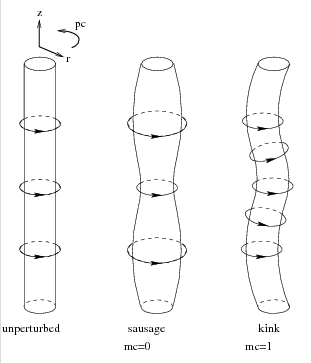
\includegraphics[width=1.5in]{kink_saus.png}}
    \end{columns}
\end{frame}


\begin{frame}{My Research}
\end{frame}

\end{document}
